\documentclass[preview]{standalone}
\usepackage{amsmath}
\usepackage{tikz}
\usepackage{mathdots}
\usepackage{yhmath}
\usepackage{cancel}
\usepackage{color}
\usepackage{xcolor}
\usepackage{siunitx}
\usepackage{array}
\usepackage{multirow}
\usepackage{amssymb}
\usepackage{gensymb}
\usepackage{tabularx}
\usepackage{extarrows}
\usepackage{booktabs}
\usetikzlibrary{fadings}
\usetikzlibrary{patterns}
\usetikzlibrary{shadows.blur}
\usetikzlibrary{shapes}
\begin{document}
\begin{center}



\tikzset{every picture/.style={line width=0.75pt}} %set default line width to 0.75pt        

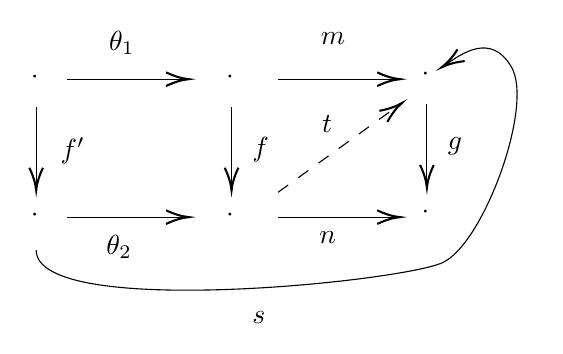
\begin{tikzpicture}[x=0.75pt,y=0.75pt,yscale=-1,xscale=1]
%uncomment if require: \path (0,169); %set diagram left start at 0, and has height of 169

%Straight Lines [id:da8409702886460745] 
\draw    (233.2,31.94) -- (289.92,31.94) ;
\draw [shift={(291.92,31.94)}, rotate = 180] [color={rgb, 255:red, 0; green, 0; blue, 0 }  ][line width=0.75]    (10.93,-3.29) .. controls (6.95,-1.4) and (3.31,-0.3) .. (0,0) .. controls (3.31,0.3) and (6.95,1.4) .. (10.93,3.29)   ;
%Straight Lines [id:da16004951314787053] 
\draw    (334.94,31.94) -- (391.66,31.94) ;
\draw [shift={(393.66,31.94)}, rotate = 180] [color={rgb, 255:red, 0; green, 0; blue, 0 }  ][line width=0.75]    (10.93,-3.29) .. controls (6.95,-1.4) and (3.31,-0.3) .. (0,0) .. controls (3.31,0.3) and (6.95,1.4) .. (10.93,3.29)   ;
%Straight Lines [id:da5842840994613554] 
\draw    (233.2,98.4) -- (289.92,98.4) ;
\draw [shift={(291.92,98.4)}, rotate = 180] [color={rgb, 255:red, 0; green, 0; blue, 0 }  ][line width=0.75]    (10.93,-3.29) .. controls (6.95,-1.4) and (3.31,-0.3) .. (0,0) .. controls (3.31,0.3) and (6.95,1.4) .. (10.93,3.29)   ;
%Straight Lines [id:da7865994793652886] 
\draw    (334.94,98.4) -- (391.66,98.4) ;
\draw [shift={(393.66,98.4)}, rotate = 180] [color={rgb, 255:red, 0; green, 0; blue, 0 }  ][line width=0.75]    (10.93,-3.29) .. controls (6.95,-1.4) and (3.31,-0.3) .. (0,0) .. controls (3.31,0.3) and (6.95,1.4) .. (10.93,3.29)   ;
%Straight Lines [id:da4220078450679592] 
\draw    (218.41,45.23) -- (218.41,83.55) ;
\draw [shift={(218.41,85.55)}, rotate = 270] [color={rgb, 255:red, 0; green, 0; blue, 0 }  ][line width=0.75]    (10.93,-3.29) .. controls (6.95,-1.4) and (3.31,-0.3) .. (0,0) .. controls (3.31,0.3) and (6.95,1.4) .. (10.93,3.29)   ;
%Straight Lines [id:da3145760408714827] 
\draw    (312.53,45.23) -- (312.53,83.55) ;
\draw [shift={(312.53,85.55)}, rotate = 270] [color={rgb, 255:red, 0; green, 0; blue, 0 }  ][line width=0.75]    (10.93,-3.29) .. controls (6.95,-1.4) and (3.31,-0.3) .. (0,0) .. controls (3.31,0.3) and (6.95,1.4) .. (10.93,3.29)   ;
%Straight Lines [id:da5084674615365148] 
\draw    (406.66,43.9) -- (406.66,82.23) ;
\draw [shift={(406.66,84.23)}, rotate = 270] [color={rgb, 255:red, 0; green, 0; blue, 0 }  ][line width=0.75]    (10.93,-3.29) .. controls (6.95,-1.4) and (3.31,-0.3) .. (0,0) .. controls (3.31,0.3) and (6.95,1.4) .. (10.93,3.29)   ;
%Curve Lines [id:da955156656570751] 
\draw    (218.41,114.36) .. controls (218.67,147.66) and (394.61,129.59) .. (414.33,120.28) .. controls (434.05,110.97) and (458.2,44.79) .. (447.44,26.18) .. controls (437.44,8.87) and (422.87,20.11) .. (415.39,25.16) ;
\draw [shift={(413.83,26.18)}, rotate = 328.29] [color={rgb, 255:red, 0; green, 0; blue, 0 }  ][line width=0.75]    (10.93,-3.29) .. controls (6.95,-1.4) and (3.31,-0.3) .. (0,0) .. controls (3.31,0.3) and (6.95,1.4) .. (10.93,3.29)   ;
%Straight Lines [id:da5099104984645619] 
\draw  [dash pattern={on 4.5pt off 4.5pt}]  (334.94,86.44) -- (392.93,44.63) ;
\draw [shift={(394.55,43.46)}, rotate = 144.21] [color={rgb, 255:red, 0; green, 0; blue, 0 }  ][line width=0.75]    (10.93,-3.29) .. controls (6.95,-1.4) and (3.31,-0.3) .. (0,0) .. controls (3.31,0.3) and (6.95,1.4) .. (10.93,3.29)   ;

% Text Node
\draw (214.58,26.68) node [anchor=north west][inner sep=0.75pt]    {$\cdot $};
% Text Node
\draw (214.58,93.15) node [anchor=north west][inner sep=0.75pt]    {$\cdot $};
% Text Node
\draw (308.71,26.68) node [anchor=north west][inner sep=0.75pt]    {$\cdot $};
% Text Node
\draw (308.71,93.15) node [anchor=north west][inner sep=0.75pt]    {$\cdot $};
% Text Node
\draw (402.83,25.35) node [anchor=north west][inner sep=0.75pt]    {$\cdot $};
% Text Node
\draw (402.83,91.82) node [anchor=north west][inner sep=0.75pt]    {$\cdot $};
% Text Node
\draw (252.27,7.39) node [anchor=north west][inner sep=0.75pt]    {$\theta _{1}$};
% Text Node
\draw (250.92,105.76) node [anchor=north west][inner sep=0.75pt]    {$\theta _{2}$};
% Text Node
\draw (354.28,8.39) node [anchor=north west][inner sep=0.75pt]    {$m$};
% Text Node
\draw (353.59,104.1) node [anchor=north west][inner sep=0.75pt]    {$n$};
% Text Node
\draw (415.45,58.9) node [anchor=north west][inner sep=0.75pt]    {$g$};
% Text Node
\draw (321.32,58.9) node [anchor=north west][inner sep=0.75pt]    {$f$};
% Text Node
\draw (228.89,58.9) node [anchor=north west][inner sep=0.75pt]    {$f'$};
% Text Node
\draw (321.32,142.82) node [anchor=north west][inner sep=0.75pt]    {$s$};
% Text Node
\draw (354.94,48.27) node [anchor=north west][inner sep=0.75pt]    {$t$};

\end{tikzpicture}

\end{center}
\end{document}
